\section{Link analysis}
\subsection{Introduction}
\textbf{Early search engines} retrieved \textbf{relevant pages} for the user based primarily on the content \textbf{similarity} of the user \textbf{query} and the \textbf{indexed pages} of the search engines. Starting from \textbf{1996}, it became clear that \textbf{content similarity} alone was \textbf{no longer sufficient} for search due to two reasons:

\begin{enumerate}
    \item The \textbf{number of Web pages grew rapidly} during the middle to late 1990s. Given any query, the number of relevant pages can be huge, and this abundance of information causes a major problem for ranking, i.e., how to choose only 10–30 pages and rank them suitably to present to the user;
    \item Content \textbf{similarity methods} are easily \textbf{spammed}. A page owner can \textbf{repeat some important words} and add many remotely related words in his/her pages to \textbf{boost the rankings of the pages} and/or to make the pages relevant to a large number of possible queries.
\end{enumerate}

Starting from around 1996, researchers in academia and search engine companies began to work on the problem, and they resorted to \textbf{hyperlinks}. Unlike \textbf{text documents} used in traditional information retrieval, which are often considered \textbf{independent} of one another (i.e., with no explicit relationships or links among them except in citation analysis), \textbf{Web pages} are \textbf{connected} through \textbf{hyperlinks}, which carry important information. \textbf{Some} hyperlinks are used to \textbf{organize} a large amount of information at the same Web site, and thus \textbf{only point to pages in the same site}. \textbf{Other} hyperlinks point to \textbf{pages in other Web sites}. Such out-going hyperlinks often indicate an implicit conveyance of authority to the pages being pointed to. Therefore, those \textbf{pages} that are \textbf{pointed to} by \textbf{many other pages} are likely to \textbf{contain authoritative or quality information}. Such linkages should obviously be used in page evaluation and ranking in search engines. 

During the period of 1997-1998, two most influential hyperlink based search algorithms \textbf{PageRank} and \textbf{HITS} were designed. PageRank is the algorithm that powers the successful search engine Google. Both PageRank and HITS were originated from \textbf{social network analysis},and they both exploit the hyperlink structure of the Web to rank pages according to their levels of “prestige” or “authority”. 

Notice that apart from search ranking, hyperlinks are also useful for \textbf{finding Web communities}. A Web community is a cluster of densely linked pages representing a group of people with a common interest. Beyond explicit hyperlinks on the Web, explicit or implicit links in other contexts are useful too, e.g., for discovering communities of named entities (e.g., people and organizations) in free text documents and for analyzing social phenomena in emails and friendship networks on social networking sites.

\subsection{Network properties}
Before analyzing the two algorithms defined above, we now focus on some important properties of \textbf{networks}, in particular the one of the Web graph. 

A network is defined as \textbf{scale-free} if its degree distribution, i.e. the probability $P(k_i)$ that a node selected uniformly at random has $k_i$ degree, follows a \textbf{power law} distribution:

$$
P(k_i) = c \cdot k_i ^{-\alpha}
$$

Picture \ref{random vs scale free} shows the difference between a random network and a scale-free network.

\begin{figure}[h!]
		\centering
		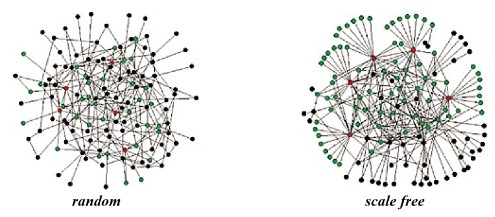
\includegraphics[scale = 1.8]{img/random vs scale free.jpg}
		\label{random vs scale free}
        \caption{Random vs scale-free network}
\end{figure}

In other word, the property of scale-free networks ensures that:

\begin{itemize}
    \item The \textbf{ratio} of very \textbf{connected nodes} and the number of nodes in the rest of the network remains \textbf{constant} as the network changes in size;
    \item Scale-free networks may show almost \textbf{no degradation} as "random" nodes fail: if failures occur randomly, since most nodes have a small degree, the likelihood that a hub (with many links) would be affected is almost negligible. But such networks highly \textbf{suffer from attacks toward high degree nodes}, which may cause disasters in the global inter-connectivity;
    \item They have a high value of the so-called \textbf{clustering coefficient} $C$. Given a vertex $v$, let $k_v$ be the number of neighbors of $v$, then $C_v = \frac{\text{# existing links}}{\text{# all possible existing links}} = \frac{\text{# existing links}}{k_v (k_v - 1)}$. Then $C$ is computed as the average across all the values of $C_v$. This coefficient in scale-free networks is about five times higher than the coefficient of a random graph. Notice that, in general, the coefficient decreases as the node degrees increase.
\end{itemize}

Notice that the name of scale-free networks comes from the fact that the power-law distribution looks the same, no matter the scale of the network. In this sense, the \textbf{shape} of the power-law \textbf{distribution} remains \textbf{unchanged}, except for a multiplicative constant. From a mathematical point of view, a probability distribution $p(x)$ is scale-free if exists $g(b)$ s.t. $p(bx) = g(b) p(x)$, for each $b$ and $x$. If we consider the power-law distribution $p(x) = c \cdot x^{-\alpha}$:

$$
p(bx) = c \cdot (bx)^{-\alpha} = b^{-\alpha} \cdot c \cdot x^{-\alpha}
$$

from which we derive that $g(b) = b^{-\alpha}$, so that the property $p(bx) = g(b) p(x)$ is ensured.

Scale-free networks arise from the \textbf{preferential attachment process}, a pattern of network growth in which new nodes prefer to link to highly connected nodes. In other words, given a new node, the probability that it connects to $\text{node}_i$ is proportional to the number of existing links $k_i$ to $\text{node}_i$:

$$
P(\text{linking to node}_i) = \frac{k_i}{\sum_j k_j}
$$

If we think of a citation network, we are more likely to cite pages that already have a lot of links, and hence there's a positive feedback loop.

Finally, one last property on the Web network is that is is a \textbf{small world}, i.e. it has a short average path length $d$: in particular, $d = 0.35 + 2.06 \log N$. If we consider $N = 8 * 10^8$, then $d = 18.59$, i.e. two randomly chosen documents on the Web are on average 19 clicks away from each other.

\subsection{Social network analysis}
Social network is the study of \textbf{social entities} and their interactions and \textbf{relationships}. The interactions and \textbf{relationships} can be \textbf{represented} with a network or \textbf{graph}, where each vertex (or node) represents an actor and each link represents a relationship. From the network we can study the \textbf{properties of its structure}, and the role, position and prestige of each social actor. We can also find various kinds of sub-graphs, e.g., \textbf{communities} formed by groups of actors. 

Social network analysis is useful for the Web because the Web is essentially a virtual society, and thus a virtual social network, where each page can be regarded as a social actor and each hyperlink as a relationship.

In this section, we introduce two types of social network analysis, \textbf{centrality} and \textbf{prestige}, which are closely related to hyperlink analysis and search on the Web. Both centrality and prestige are \textbf{measures of degree of prominence of an actor in a social network}. 

\subsubsection{Centrality}
\textbf{Important} or prominent actors are those that are \textbf{linked} or involved with \textbf{other actors extensively}. In the context of an organization, a person with extensive contacts (links) or communications with many other people in the organization is considered more important than a person with relatively. A \textbf{central node} is a node involved in \textbf{many relationships}.

There are different types of links or involvements between actors. Thus, several types of centrality are defined on undirected and directed graphs. We discuss three popular types below.

\underline{\textbf{Degree centrality}}

Let the total number of actors in the network be $n$. In an \textbf{undirected graph}, the degree centrality of an actor $i$ (denoted by $C_D(i)$) is simply the \textbf{node degree} (the number of edges) of the actor node, denoted by $d(i)$, \textbf{normalized} with the \textbf{maximum degree}, $n-1$:

$$
C_D(i) = \frac{d(i)}{n-1}
$$

Notice that $0 \leq C_D(i) \leq 1$.

In a \textbf{directed graph}, we need to distinguish \textbf{in-links} of actor $i$ (links pointing to i), and \textbf{out-links} (links pointing out from $i$). The degree centrality is defined based on only the out-degree (the number of out-links or edges), $d_o(i)$:

$$
C'_D(i) = \frac{d_o(i)}{n-1}
$$

\underline{\textbf{Closeness centrality}}

This view of centrality is based on the closeness or \textbf{distance}. The basic idea is that an \textbf{actor} $xi$ is \textbf{central} if it can \textbf{easily interact} with \textbf{all other actors}. That is, its \textbf{distance to all other actors is short}. Thus, we can use the shortest distance to compute this measure. 

Let the shortest distance from actor $i$ to actor $j$ be $d(i, j)$ (measured as the number of links in a shortest path): then, for an undirected graph the closeness centrality $C_C(i)$ of actor $i$ is defined as 

$$
C_C(i) = \frac{n-1}{\sum_{j = 1}^n d(i,j)}
$$

Notice that in this case we're assuming that the graph is connected, i.e. there exists a path from any point to any other point s.t. $d(i,j) \geq 0$. Also in this case $0 \leq C_C(i) \leq 1$.

The \textbf{same equation} can be used for a \textbf{directed graph}. 

\underline{\textbf{Betweenness centrality}}

If two non-adjacent actors $j$ and $k$ want to interact and actor $i$ is on the path between $j$ and $k$, then $i$ may have some control over their interactions. Betweenness measures this \textbf{control of $i$ over other pairs of actors}. Thus, if $i$ is on the \textbf{paths} of \textbf{many} such \textbf{interactions}, then $i$ is an \textbf{important actor.}

For an \textbf{undirected graph}, let $p_{jk}$ be the number of shortest paths between actors $j$ and $k$. The betweenness of an actor $i$ is defined as the number of shortest paths that pass $i$ (denoted by $p_{jk}(i)$, $j \neq i$ and $k \neq i$) normalized by the total number of shortest paths of all pairs of actors not including $i$:

$$
C_B(i) = \sum_{j < k} \frac{p_{jk}(i)}{p_{jk}}
$$

Note that there may be multiple shortest paths between actor $j$ and actor $k$. Some pass $i$ and some do not. We assume that all paths are equally likely to be used. $C_B(i)$ has a \textbf{minimum} of 0, attained when $i$ falls on no shortest path. Its \textbf{maximum} is $(n-1)(n-2)/2$, which is the number of pairs of actors not including $i$. In the network of Picture \ref{bet}, actor 1 is the most central actor. It lies on all 15 shortest paths linking the other 6 actors. $C_B(1)$ has the maximum value of 15, and $C_B(2) = C_B(3) = C_B(4) = C_B(5) = C_B(6) = C_B(7) = 0$.

\begin{figure}[h!]
		\centering
		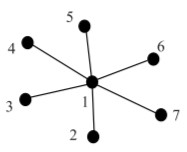
\includegraphics[scale = 1.8]{img/betweenness.jpg}
		\label{bet}
        \caption{Betweenness centrality}
\end{figure}

If we are to ensure that the value range is between 0 and 1, we can normalize it with $(n-1)(n-2)/2$, which is the maximum value of $C_B(i)$. The standardized betweenness of actor $i$ is defined as:

$$
C'_B(i) = \frac{2 \sum_{j < k} \frac{p_{jk}(i)}{p_{jk}}}{(n-1)(n-2)}
$$

Unlike the closeness measure, the betweenness can be computed even if the graph is not connected.

For a \textbf{directed graph}, the same equation can be used but must be multiplied by 2 because there are now $(n-1)(n-2)$ pairs considering a path from $j$ to $k$ is different from a path from $k$ to $j$.

\subsubsection{Prestige}
\textbf{Prestige} is a \textbf{more refined measure of prominence} of an actor than centrality as we will see below. We need to distinguish between ties sent (\textbf{out-links}) and ties received (\textbf{in-links}), and to compute the \textbf{prestige} of an actor, we only look at the \textbf{in-links}. Hence, the prestige cannot be computed unless the relation is directional or the graph is directed. The main difference between the concepts of centrality and prestige is that \textbf{centrality} focuses on \textbf{out-links} while \textbf{prestige} focuses on \textbf{in-links}. 

We define three prestige measures. The third prestige measure (i.e., rank prestige) forms the basis of most Web page link analysis algorithms, including PageRank and HITS.

\underline{\textbf{Degree prestige}}

Based on the definition of the prestige, it is clear that an actor is \textbf{prestigious} if it \textbf{receives many in-links} or nominations. Thus, the simplest measure of prestige of an actor $i$ (denoted by $P_D(i)$) is its in-degree,

$$
P_D(i) = \frac{d_I(i)}{n-1}
$$

where $d_I(i)$ is the in-degree of $i$ (the number of in-links of $i$) and $n - 1$ is the maximum in-degree of a node. As in the degree centrality, dividing by $n - 1$ standardizes the prestige value to the range from 0 and 1. The \textbf{maximum} prestige value is 1 when \textbf{every other actor links to or chooses actor $i$}.

\underline{\textbf{Proximity prestige}}

The degree prestige of an actor $i$ only considers the actors that are adjacent to $i$. The proximity prestige \textbf{generalizes} it by \textbf{considering} both the \textbf{actors directly and indirectly linked to actor} $i$. That is, we consider every actor $j$ that can reach $i$, i.e., there is a directed path from $j$ to $i$. 

Let $I_i$ be the set of actors that can reach actor $i$ (notice that $|I_i| \leq 1$). The \textbf{proximity} is defined as \textbf{closeness} or distance of \textbf{other actors to $i$}. Let $d(j, i)$ denote the shortest path distance from actor $j$ to actor $i$: to compute the proximity prestige, we use the average distance, which is

$$
\sum_{j \in I_i} \frac{d(j,i)}{|I_i|}
$$

If we look at the \textbf{ratio} or proportion of \textbf{actors} who \textbf{can reach $i$} to the \textbf{average distance that these actors are from $i$}, we obtain the \textbf{proximity prestige}, which has the value range of [0, 1]:

$$
P_P(i) = \frac{\frac{|I_i|}{n-1}}{\sum_{j \in I_i} \frac{d(j,i)}{|I_i|}}
$$

where $|I_i|/(n-1)$ is the \textbf{proportion} of \textbf{actors} that \textbf{can reach actor $i$}. In one extreme, every actor can reach actor $i$, which gives $|I_i|/(n-1) = 1$. The denominator is 1 if every actor is adjacent to $i$. Then, $P_P(i) = 1$. On the other extreme, no actor can reach actor i. Then $|I_i| = 0$, and $P_P(i) = 0$.

\underline{\textbf{Rank prestige}}

The above two prestige measures are based on in-degrees and distances. However, an important factor that has not been considered is the prominence of individual actors who do the “voting” or “choosing.” In the \textbf{real world}, a \textbf{person} $i$ \textbf{chosen} by an \textbf{important person} is \textbf{more prestigious} than chosen by a less important person. If one’s circle of influence is full of prestigious actors, then one’s own prestige is also high. Thus one’s \textbf{prestige} is \textbf{affected} by the \textbf{ranks or statuses of the involved actors}. Based on this intuition, the rank prestige $P_R(i)$ is defined as a \textbf{linear combination of links that point to $i$}:

$$
P_R(i) = \sum_{j = 1}^n A_{ji} \cdot P_R(j)
$$

where $A_{ji} = 1$ if $j$ points to $i$, and 0 otherwise. This equation says that an \textbf{actor’s rank prestige} is a \textbf{function} of the \textbf{ranks of the actors who vote or choose the actor}, which makes perfect sense. 

Since we have $n$ equations for $n$ actors, we can write them in the \textbf{matrix notation}. We use $P$ to represent the \textbf{column vector} that contains all the rank prestige values, i.e., $P = (P_R(1), P_R(2), …, P_R(n))^T$. We use matrix $A$ (where $A_{ij} = 1$ if $i$ points to $j$, and 0 otherwise) to represent the \textbf{adjacency matrix} of the network or graph. Then, we have

$$
P = A^T P
$$

This equation is precisely the \textbf{characteristic equation} used for finding the \textbf{eigensystem} of the matrix $A^T$, so \textbf{$P$} is an \textbf{eigenvector} of $A^T$. 

This equation and the idea behind it turn out to be very useful in Web search. Indeed, the most well known ranking algorithms for Web search, PageRank and HITS, are directly related to this equation. 

\subsection{Co-Citation and Bibliographic Coupling}
Another area of research concerned with links is the \textbf{citation analysis} of scholarly publications. A scholarly publication usually cites related prior work to acknowledge the origins of some ideas in the publication and to compare the new proposal with existing work. Citation analysis is an area of bibliometric research, which \textbf{studies} \textbf{citations} to \textbf{establish} the \textbf{relationships} between \textbf{authors and their work}.

When a publication (also called a paper) cites another publication, a relationship is established between the publications. Citation analysis uses these relationships (links) to perform various types of analysis. A \textbf{citation} can represent many types of \textbf{links}, such as links between \textbf{authors}, \textbf{publications}, \textbf{journals} and conferences, and fields, or even between countries. We will discuss two specific types of citation analysis, co-citation and bibliographic coupling. 

\subsubsection{Co-citation}
\textbf{Co-citation} is used to \textbf{measure} the \textbf{similarity} of \textbf{two papers}. If papers $i$ and $j$ are both cited by paper $k$, then they may be said to be related in some sense to each other, even though they do not directly cite each other. Picture \ref{co cit} shows that papers $i$ and $j$ are co-cited by paper $k$. If papers $i$ and $j$ are cited together by many papers, it means that $i$ and $j$ have a strong relationship or similarity. The \textbf{more papers they are cited by}, the \textbf{stronger} their \textbf{relationship} is.

\begin{figure}[h!]
		\centering
		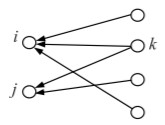
\includegraphics[scale = 1.8]{img/co-citation.jpg}
		\label{co cit}
        \caption{Co-citation}
\end{figure}

Let $L$ be the \textbf{citation matrix}, where $L_{ij} = 1 $ if paper $i$ cites paper $j$, and 0 otherwise. \textbf{Co-citation} (denoted by $C_{ij}$) is a \textbf{similarity measure} defined as the \textbf{number of papers that co-cite $i$ and $j$}, and is computed with

$$
C_{ij} = \sum_{k = 1}^n L_{ki}L_{kj} = (L^T L)_{ij}
$$

where $n$ is the total number of papers. Notice that $C_{ii}$ is naturally the number of papers that cite $i$. A square matrix $C$ can be formed with $Cij$, and it is called the \textbf{co-citation matrix}. Co-citation is symmetric, $C_{ij} = C_{ji}$, and is commonly \textbf{used} as a \textbf{similarity measure} of two \textbf{papers} in \textbf{clustering} to group papers of similar topics together.

\subsubsection{Bibliographic coupling}
\textbf{Bibliographic coupling} operates on a similar principle, but in a way it is the \textbf{mirror image of co-citation}. Bibliographic coupling \textbf{links} \textbf{papers} that \textbf{cite the same articles} so that if papers $i$ and $j$ both cite paper $k$, they may be said to be related, even though they do not directly cite each other. The \textbf{more papers they both cite}, the \textbf{stronger} their \textbf{similarity} is. Picture \ref{bib coup} shows both papers $i$ and $j$ citing (referencing) paper $k$.

\begin{figure}[h!]
		\centering
		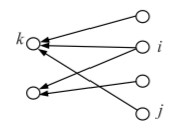
\includegraphics[scale = 1.8]{img/biblio coupling.jpg}
		\label{bib coup}
        \caption{Bibliographic coupling}
\end{figure}

We use $B_{ij}$ to represent the number of papers that are cited by both
papers $i$ and $j$: 

$$
B_{ij} = \sum_{k = 1}^n L_{ik}L_{jk} = (LL^T)_{ij}
$$

$B_{ii}$ is naturally the \textbf{number of references} (in the reference list) of paper $i$. A \textbf{square matrix $B$} can be formed with $B_{ij}$, and it is called the \textbf{bibliographic coupling matrix}. Bibliographic coupling is also \textbf{symmetric} and is regarded as a similarity measure of two papers in clustering. We will see later that two important types of pages on the Web, hubs and authorities, found by the HITS algorithm are directly related to co-citation and bibliographic coupling matrices.

\subsection{PageRank}
The year 1998 was an important year for Web link analysis and Web search, since both the PageRank and the HITS algorithms were reported in that year. The main ideas of PageRank and HITS are really quite similar. However, it is their dissimilarity that made a huge difference as we will see later. Since that year, \textbf{PageRank} has emerged as the \textbf{dominant} \textbf{link analysis model} for Web search, partly due to its \textbf{query-independent evaluation of Web pages} and its \textbf{ability} to \textbf{combat spamming}, and partly due to Google’s business success. 

PageRank relies on the \textbf{democratic nature of the Web} by using its vast link structure as an indicator of an individual page's quality. In essence, PageRank interprets a \textbf{hyperlink} from page $x$ to page $y$ as a \textbf{vote}, by page $x$, for page $y$. However, PageRank looks at \textbf{more than just the sheer number of votes} or links that a page receives. It also analyzes the \textbf{page} that \textbf{casts} the vote. \textbf{Votes} casted by pages that are themselves\textbf{ “important”} weigh more heavily and help to make other pages more “important.” This is exactly the idea of rank prestige in social networks.

\subsubsection{PageRank algorithm}
PageRank is a \textbf{static ranking of Web pages} in the sense that a \textbf{PageRank} value is \textbf{computed for each page off-line} and it does \textbf{not depend on search queries}. Since PageRank is based on the measure of prestige in social networks, the \textbf{PageRank value} of each page can be regarded as its \textbf{prestige}.

From the perspective of prestige, we use the following to derive the PageRank algorithm:

\begin{enumerate}
    \item A \textbf{hyperlink} from a \textbf{page} pointing \textbf{to} another \textbf{page} is an implicit conveyance of authority to the target page. Thus, the \textbf{more in-links} that a page $i$ receives, the \textbf{more prestige} the page $i$ has;
    \item Pages that point to page $i$ also have their own prestige scores. A page with a \textbf{higher prestige} score \textbf{pointing} to $i$ is \textbf{more important} than a page with a \textbf{lower prestige} score pointing to $i$. In other words, a \textbf{page} is \textbf{important} if it is \textbf{pointed} to by other \textbf{important pages}.
\end{enumerate}

According to rank prestige in social networks, the importance of page $i$ ($i$’s \textbf{PageRank score}) is \textbf{determined} by \textbf{summing up the PageRank scores of all pages that point to $i$}. Since a page may point to many other pages, its \textbf{prestige score should be shared among all the pages} that it points to. Notice the difference from rank prestige, where the prestige score is not shared.

To formulate the above ideas, we treat the Web as a directed graph $G =
(V, E)$, where $V$ is the set of vertices or nodes, i.e., the set of all pages, and $E$ is the set of directed edges in the graph, i.e., hyperlinks. Let the total number of pages on the Web be $n$ (i.e., $n = |V|$). The PageRank score of the page $i$ (denoted by $P(i)$) is defined by:

\begin{equation}\label{PageRank}
    P(i) = \sum_{(j,i) \in E} \frac{P(j)}{O_j}
\end{equation}

, where $O_j$ is the number of out-links of page j, and it represents the "quantity" of prestige which is spread among the neighbors of $i$.

Mathematically, we have a system of $n$ linear equations with $n$ unknowns, so we can use a \textbf{matrix} to represent \textbf{all the equations}. Let $P$ be a $n$-dimensional column vector of PageRank values, i.e., 

$$
P = (P(1), P(2), …, P(n))^T
$$

Let $A$ be the adjacency (usually sparse) matrix of our graph with

$$
A_{ij} = \begin{cases}
    \frac{1}{O_i} \qquad \text{if } (i,j) \in E \\
    0 \qquad \text{otherwise}
\end{cases}
$$

We can write the system of $n$ equations with as

\begin{equation}\label{PageRank matrix}
    P = A^T P
\end{equation}

This is the \textbf{characteristic equation of the eigensystem}, where the \textbf{solution to P} is an \textbf{eigenvector} with the corresponding \textbf{eigenvalue of 1} ($\lambda = 1$). Since this is a \textbf{circular definition}, an \textbf{iterative algorithm is used to solve it}. It turns out that if \textbf{some conditions} are satisfied (which will be described shortly), \textbf{1 is the largest eigenvalue} and the \textbf{PageRank vector $P$ is the principal eigenvector}. A well known mathematical technique called \textbf{power iteration} can be used to find $P$:

$$
P_k = A^T P_{k-1}
$$

Notice that the power iteration method stops when $P_k \approx P_{k-1}$. 

However, the problem is that Equation \ref{PageRank matrix} does not quite suffice because the Web graph does not meet the conditions. To introduce these conditions and the enhanced equation, let us derive the same Equation based on the \textbf{Markov chain}. In the Markov chain model, \textbf{each Web page} or node in the Web graph is \textbf{regarded as a state}. A \textbf{hyperlink} is a \textbf{transition}, which leads \textbf{from one state to another state with a probability}. Thus, this framework models \textbf{Web surfing as a stochastic process}. It models a Web surfer randomly surfing the Web as a state transition in the Markov chain. Recall that we used $O_i$ to denote the number of out-links of a node $i$. Each \textbf{transition probability is $1/O_i$} if we assume the Web surfer will click the hyperlinks in the page $i$ \textbf{uniformly} at random, the “back” button on the browser is not used and the surfer does not type in an URL. Let $A$ be the state transition probability matrix, a square matrix of the following format:

$$
A = \begin{bmatrix}
A_{11} & A_{12} & \hdots & A_{1n}\\
A_{21} & A_{22} & \hdots & A_{2n}\\
\vdots & \vdots & \ddots & \vdots\\
A_{n1} & A_{n2} & \hdots  & A_{nn} 
\end{bmatrix}
$$

, where $A_{ij}$ represents the \textbf{transition probability} that the \textbf{surfer} in \textbf{state} $i$ (page $i$) will move to \textbf{state} $j$ (page $j$). 

Given an \textbf{initial probability distribution vector} that a surfer is at each state (or page) $p_0 = (p_0(1), p_0(2), …, p_0(n))^T$ (a column vector) and an $n \times n$ transition probability matrix $A$, we have

\begin{equation}
    \sum_{i = 1}^n p_0(i) = 1
\end{equation}

\begin{equation}\label{Sum of the rows equal to 1}
    \sum_{j = 1}^n A_{ij} = 1
\end{equation}

Equation \ref{Sum of the rows equal to 1} is not quite true for some Web pages because they have no out-links. If the matrix $A$ satisfies Equation \ref{Sum of the rows equal to 1}, we say that $A$ is the \textbf{stochastic matrix of a Markov chain}. Let us assume $A$ is a stochastic matrix for the time being and deal with it not being that later. 

In a Markov chain, a question of common interest is: \textbf{given the initial probability distribution} $p_0$ at the beginning, what is the \textbf{probability} that $m$ \textbf{steps}/transitions later that the \textbf{Markov chain will be at each state} $j$? We can determine the probability that the system (or the random surfer) is in state $j$ after 1 step (1 state transition) by using the following reasoning:

$$
p_1(j) = \sum_{i = 1}^n A_{ij}(1) p_0(i)
$$

where $A_{ij}(1)$ is the probability of going from $i$ to $j$ in 1 transition, and $A_{ij}(1) = A_{ij}$. We can write it with a matrix:

$$
p_1 = A^T p_0
$$

In general, the probability distribution after $k$ steps is:

\begin{equation}
    p_k = A^T p_{k-1}
\end{equation}

By the \textbf{Ergodic Theorem of Markov chains}, a \textbf{finite Markov chain} defined by the stochastic transition matrix $A$ has a \textbf{unique stationary probability distribution} if $A$ \textbf{is irreducible and aperiodic}. 

The \textbf{stationary probability distribution} means that \textbf{after a series of transitions} $p_k$ w\textbf{ill converge to a steady-state probability vector} $\pi$ \textbf{regardless of the choice of the initial probability vector} $p_0$, i.e.,

$$
\lim_{k \to \infty} p_k = \pi
$$

When we reach the steady-state, we have $p_k = p_{k+1} = \pi$, and thus $\pi = A^T \pi$. $\pi$ is the \textbf{principal eigenvector} of $A^T$ with \textbf{eigenvalue} \textbf{of 1}. In PageRank, $\pi$ is used as the PageRank vector $P$. Thus, we obtain:

\begin{equation}\label{Ideal PR equation}
    P = A^T P
\end{equation}

Using the \textbf{stationary probability distribution} $\pi$ as the \textbf{PageRank vector} is \textbf{reasonable} and quite \textbf{intuitive} because it reflects the long-run probabilities that a random surfer will visit the pages. A page has a high prestige if the probability of visiting it is high.

Now let us come back to the real Web context and \textbf{see whether the above conditions are satisfied}, i.e., whether $A$ is a stochastic matrix and whether it is irreducible and aperiodic. In fact, none of them is satisfied. Hence, we need to \textbf{extend} the ideal-case Equation \ref{Ideal PR equation} to produce the \textbf{“actual PageRank model”}. Let us look at each condition below. 

First of all, $A$ is \textbf{not a stochastic} (transition) \textbf{matrix}. A stochastic matrix is the transition matrix for a finite Markov chain whose entries in each row are non-negative real numbers and sum up to 1. This requires that \textbf{every Web page must have at least one out-link}. This is \textbf{not true on the Web because many pages have no out-links}, which are reflected in transition matrix $A$ by \textbf{some rows of complete 0’s}. Such pages are called the \textbf{dangling pages (nodes)}.

\underline{Example: Dangling node in a graph}: as we can see, Picture \ref{dangling} shows that node 5 is a dangling node, and the corresponding transition matrix is not a stochastic matrix.

\begin{figure}[h!]
		\centering
		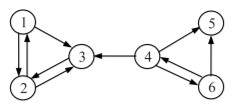
\includegraphics[scale = 1.8]{img/dangling node.jpg}
        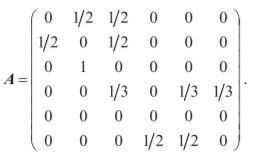
\includegraphics[scale = 1.8]{img/dangling node matrix.jpg}
		\label{dangling}
        \caption{Example of dangling node}
\end{figure}

We can fix this problem in several ways in order to convert A to a stochastic transition matrix. We describe only two ways here:

\begin{enumerate}
    \item \textbf{Remove} those \textbf{pages} with \textbf{no out-links} from the system \textbf{during the PageRank computation} as these pages do not affect the ranking of any other page directly. Out-links from other pages pointing to these pages are also removed. After PageRanks are computed, these pages and hyperlinks pointing to them can be added in. Note that the \textbf{transition probabilities} of those pages with removed links will be \textbf{slightly affected} but not significantly;
    \item \textbf{Add} a \textbf{complete set of outgoing links} \textbf{from} \textbf{each such page} $i$ \textbf{to all the pages on the Web}. Thus the \textbf{transition probability} of going from $i$ to every page is $1/n$ assuming uniform probability distribution. That is, \textbf{we replace each row containing all 0’s} with $e/n$, where $e$ is n-dimensional vector of all 1’s.
\end{enumerate}

If we use the second method to make A a stochastic matrix by adding a
link from page 5 to every page, we obtain a stochastic matrix:

\begin{figure}[h!]
		\centering
		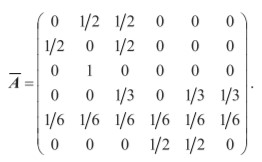
\includegraphics[scale = 1.8]{img/dangling matrix 2.jpg}
		\label{dangling2}
        \caption{Transformation of matrix $A$ into $\Bar{A}$}
\end{figure}

Second, $A$ is \textbf{not irreducible}. Irreducible means that the Web graph $G$ is \textbf{strongly connected}, i.e. if and only if, for each pair of nodes $u,v \in V$, there is a path from $u$ to $v$. A \textbf{general Web graph} represented by A is \textbf{not irreducible} because \textbf{for some pair of nodes} $u$ and $v$, \textbf{there is no path} from $u$ to $v$. For example, in Picture \ref{dangling}, there is no directed path from node 3 to node 4. The adjustment of adding a complete set of out-links is not enough to ensure irreducibility. 

Finally, $A$ is \textbf{not aperiodic}: a state $i$ in a Markov chain being \textbf{periodic} means that \textbf{there exists a directed cycle that the chain has to traverse}. More formally, a state $i$ is periodic with period $k > 1$ if $k$ is the smallest number such that all paths leading from state $i$ back to state $i$ have a length that is a multiple of $k$. If a state is not periodic (i.e., k = 1), it is aperiodic. A \textbf{Markov chain} is \textbf{aperiodic} if \textbf{all states} are \textbf{aperiodic}. 

\underline{Example: Periodic chain}: Picture \ref{periodic chain} shows a periodic Markov chain with $k = 3$. The transition matrix is given on the left. Each state in this chain has a period of 3. For example, if we start from state 1, to come back to state 1 the only path is 1-2-3-1 for some number of times, say $h$. Thus any return to state 1 will take $3h$ transitions. 

\begin{figure}[h!]
		\centering
		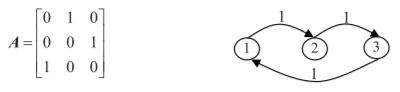
\includegraphics[scale = 1.8]{img/periodic chain.jpg}
		\label{periodic chain}
        \caption{Example of periodic chain}
\end{figure}

It is easy to deal with the above \textbf{two problems} with a single strategy, called \textbf{teleportation}: we \textbf{add} a \textbf{link} \textbf{from each page to every page} and give \textbf{each link} a \textbf{small transition probability} controlled by a \textbf{parameter} $d$, with $0 < d < 1$.

In this way, the augmented transition matrix becomes \textbf{irreducible} because it is clearly \textbf{strongly connected}. It is also \textbf{aperiodic} because the situation in Picture \ref{periodic chain} no longer exists as we now have \textbf{paths of all possible lengths from state $i$ back to state $i$}. Finally, since the augmented transition matrix is both irreducible and aperiodic, we're ensured that it has a single stationary distribution.

After this augmentation, we obtain an \textbf{improved PageRank model}. In this model, at a page, the random surfer has two options: 

\begin{enumerate}
    \item With probability $d$, he randomly chooses an out-link to follow, i.e. it \textbf{clicks on a hyperlink};
    \item With probability $1-d$, he jumps to a random page without a link.
\end{enumerate}

Thus, the improved model is

\begin{equation}
    P = ((1-d) \frac{E}{n} + dA^T) P
\end{equation}

where $E$ is $ee^T$ ($e$ is a column vector of all 1’s) and thus $E$ is a $n \times n$ square matrix of all 1’s. In this sense, $E$ represents the adjacency matrix of a completely connected graph, and we multiply it by $(1-d)/n$, which is the probability of clicking on a teleportation link.

\underline{Example: Improved PageRank model}: Picture \ref{improved model} shows the resulting matrix after applying the improved model described above. On the left we have the original matrix made stochastic, while on the left the resulting matrix. Notice that the original matrix is quite sparse, while the resulting one is dense. In this case the parameter $d = 0.9$.

\begin{figure}[h!]
		\centering
        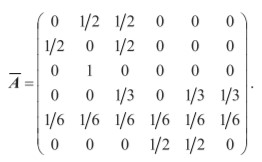
\includegraphics[scale = 1.8]{img/dangling matrix 2.jpg}
		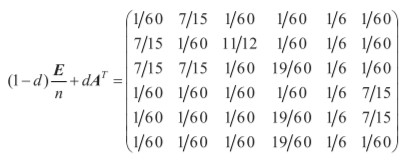
\includegraphics[scale = 1.8]{img/final matrix.jpg}
		\label{improved model}
        \caption{Resulting matrix}
\end{figure}

Notice that $(1-d) \frac{E}{n} + dA^T$ is a \textbf{stochastic matrix}, \textbf{irreducible and aperiodic}. Moreover:

$$
P = ((1-d) \frac{E}{n} + dA^T) P = (1-d)\frac{1}{n} ee^T P + dA^TP 
$$
, since $E = ee^T$ and $e^T P = 1$, since $P$ is a probability vector (i.e. it sums up to 1). For this reason, we obtain:

$$
P = (1-d)\frac{1}{n} e + dA^TP
$$

, and if we scale this equation by multiplying both sides by $n$, and considering that $e^TP = n$, then:

$$
P = (1-d)e + dA^TP
$$

This gives us the PageRank formula for each page $i$ as follows:

$$
P(i) = (1-d) + d \sum_{j = 1}^n A_{ji} P(j) = (1-d) + d \sum_{(j,i) \in E}^n \frac{P(j)}{O_j}
$$

The parameter $d$ is called \textbf{damping factor}, $0 < d < 1$, and $d = 0.85$ was used in the paper.

The computation of PageRank values of the Web pages can be done using the well known \textbf{power iteration method}, which produces the principal eigenvector with the eigenvalue of 1. The algorithm is simple, and is given in Picture \ref{pi}. 

\begin{figure}[h!]
		\centering
        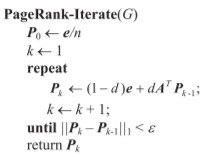
\includegraphics[scale = 1.8]{img/power iteration method.jpg}
		\label{pi}
        \caption{Power iteration method for PageRank}
\end{figure}

The iteration ends when the PageRank values do not change much or converge: in the Picture above, the iteration ends after the 1-norm of the residual vector is less than a pre-specified threshold $\epsilon$. Note that the 1-norm for a vector is simply the sum of all the components.

\underline{Example: PageRank computation}: Picture \ref{ex:page rank} shows an example of PageRank computation: in this case the PageRank equation is not scaled, so we have $e^TP = 1$ and thus $P(i) = \frac{1-d}{n} + d \sum_{(j,i) \in E} \frac{P(j)}{O_j}$.

\begin{figure}[h!]
		\centering
        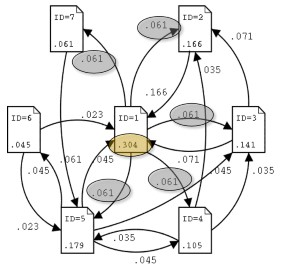
\includegraphics[scale = 1.8]{img/Example page rank.jpg}
		\label{ex:page rank}
        \caption{Example of PageRank}
\end{figure}

As we can see, the score of PageRank is written at the bottom of the page, e.g. $P(1) = 0.304$, and its score is distributed among all its 5 out-links $0.304 = 0.061 * 5$. In particular, the PageRank is obtained as $P(1) = \frac{1-d}{n} + d (0.023 + 0.166 + 0.071 + 0.045) = 0.304$, considering $d = 0.85$

\subsubsection{Advantages and disadvantages of PageRank}
The main \textbf{advantage} of PageRank is its \textbf{ability to fight spam}. A page is important if the pages pointing to it are important. Since it is \textbf{not easy} for Web page owner to \textbf{add in-links} into his/her page from other important pages, it is thus \textbf{not easy} to \textbf{influence} \textbf{PageRank}: nevertheless, there are reported ways to influence PageRank. Another major \textbf{advantage} of PageRank is that it is a \textbf{global measure} and is \textbf{query independent}. That is, the \textbf{PageRank values} of all the pages on the Web are \textbf{computed} and \textbf{saved} \textbf{off-line} \textbf{rather} than at the \textbf{query time}. At the \textbf{query time}, only a \textbf{lookup} is \textbf{needed} to find the value to be integrated with other strategies to rank the pages. It is thus \textbf{very efficient at the query time}. Both these two advantages contributed greatly to Google’s success. 

The main \textbf{criticism} is also the \textbf{query-independence} nature of PageRank. It \textbf{could not distinguish between pages that are authoritative} \textbf{in general} and pages that are \textbf{authoritative on the query topic}. Another \textbf{criticism} is that PageRank \textbf{does not consider time}, and we note again that the \textbf{link-based ranking} is \textbf{not} the \textbf{only strategy} used in a search engine. Many other information retrieval methods, heuristics, and empirical parameters are also employed. 

\subsection{HITS}
\textbf{HITS} stands for \textbf{Hypertext Induced Topic Search}. Unlike \textbf{PageRank} which is a \textbf{static} ranking algorithm, \textbf{HITS} is \textbf{search query dependent}. When the user issues a search query, \textbf{HITS} \textbf{first expands the list of relevant pages returned by a search engine} and then \textbf{produces} \textbf{two rankings} of the expanded set of pages, \textbf{authority ranking} and \textbf{hub ranking}. 

An \textbf{authority} is a \textbf{page} with \textbf{many in-links}. The idea is that the page may have \textbf{authoritative content} on some topic and thus many people trust it and thus link to it. A \textbf{hub} is a \textbf{page} with \textbf{many} \textbf{out-links}. The page serves as an \textbf{organizer of the information} on a particular topic and points to many good authority pages on the topic. When a user comes to this hub page, he/she will find many useful links which take him/her to good content pages on the topic. Picture \ref{auth and hub} shows an authority page and a hub page. 

\begin{figure}[h!]
		\centering
        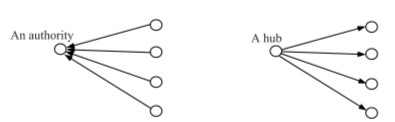
\includegraphics[scale = 1.8]{img/authorative and hub.jpg}
		\label{auth and hub}
        \caption{An authority and a hub page}
\end{figure}

The \textbf{key idea} of HITS is that a \textbf{good hub} \textbf{points} to \textbf{many good authorities} and a \textbf{good authority} is \textbf{pointed} to by \textbf{many good hubs}. Thus, authorities and hubs have a mutual reinforcement relationship. Picture \ref{auth and hub2} shows a set of densely linked authorities and hubs (a bipartite sub-graph). 

\begin{figure}[h!]
		\centering
        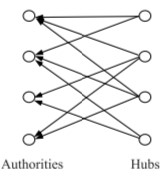
\includegraphics[scale = 1.8]{img/authorative and hub2.jpg}
		\label{auth and hub2}
        \caption{A densely linked set of authorities and hubs}
\end{figure}

Below, we first present the HITS algorithm, and also make a connection between HITS and co-citation and bibliographic coupling in bibliometric research. We then discuss the strengths and weaknesses of HITS, and describe some possible ways to deal with its weaknesses.

\subsubsection{HITS algorithm}
Before describing the HITS algorithm, let us first \textbf{describe} how \textbf{HITS} \textbf{collects} \textbf{pages} to be ranked. Given a broad search query, $q$, HITS collects a set of pages as follows: 

\begin{enumerate}
    \item It sends the \textbf{query} $q$ to a \textbf{search engine system}. It then \textbf{collects} $t$ ($t$ = 200 is used in the HITS paper) \textbf{highest ranked pages}, which assume to be highly relevant to the search query. This set is called the \textbf{root set} $W$;
    \item It then \textbf{grows} $W$ by \textbf{including} any \textbf{page pointed to by a page} in $W$ and \textbf{any page that points to a page} in $W$. This gives a larger set called $S$. However, this set can be very large. The algorithm \textbf{restricts its size} by allowing each page in $W$ to bring at most $k$ pages ($k$ = 50 is used in the HITS paper) pointing to it into $S$. The set $S$ is called the \textbf{base set}.
\end{enumerate}

HITS then works on the pages in $S$, and \textbf{assigns every page} in $S$ an \textbf{authority score} and a \textbf{hub score}. Let the number of pages to be studied be $n$. We again use $G = (V, E)$ to denote the (directed) link graph of $S$. $V$ is the set of pages (or nodes) and $E$ is the set of directed edges (or links). We use $L$ to denote the adjacency matrix of the graph:

$$
L_{ij} = \begin{cases}
    1 \qquad \text{if } (i,j) \in E \\
    0 \qquad \text{otherwise}
\end{cases}
$$

Let the \textbf{authority score} of the page $i$ be $a(i)$, and the \textbf{hub score} of page $i$ be $h(i)$. The mutual reinforcing relationship of the two scores is represented as follows:

$$
a(i) = \sum_{(j,i) \in E} h(j)
$$

, i.e. the authority score is given by the sum of the hub scores of the incoming links, and

$$
h(i) = \sum_{(i,j) \in E} a(j)
$$

, i.e. the hub score is given by the sum of the authority scores of the outgoing links.

Writing them in the \textbf{matrix form}, we use $a$ to denote the column vector with all the authority scores, $a = (a(1), a(2), …, a(n))^T$, and use $h$ to denote the column vector with all the hub scores, $h = (h(1), h(2), …, h(n))^T$:

\begin{equation}
    a = L^T h
\end{equation}

\begin{equation}
    h = La
\end{equation}

The computation of authority scores and hub scores is basically the same as the computation of the PageRank scores using the \textbf{power iteration method}. If we use $a_k$ and $h_k$ to denote authority and hub scores at the $k$-th iteration, the iterative processes for generating the final solutions are:

\begin{equation}
    a_k = L^T L a_{k-1}
\end{equation}

and

\begin{equation}
    h_k = LL^T h_{k-1}
\end{equation}

starting with $a_0 = h_0 = (1, 1, …, 1)$. After each iteration, the \textbf{values} are also \textbf{normalized} (to keep them small)
so that

$$
\sum_{i = 1}^n a(i) = 1
$$

and 

$$
\sum_{i = 1}^n h(i) = 1
$$

The algorithm is shown in Picture \ref{hits}.

\begin{figure}[h!]
		\centering
        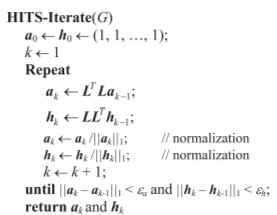
\includegraphics[scale = 1.8]{img/hits.jpg}
		\label{hits}
        \caption{HITS algorithm}
\end{figure}

The iteration ends after the 1-norms of the residual vectors are less than some thresholds $\epsilon_a$ and $\epsilon_h$. The pages with large authority and hub scores are better authorities and hubs respectively. HITS will select a few top ranked pages as authorities and hubs, and return them to the user. 

Although \textbf{HITS} will \textbf{always converge}, there is a problem with \textbf{uniqueness of limiting (converged) authority and hub vectors}. It is shown that for certain types of graphs, \textbf{different initializations} to the power method \textbf{produce} \textbf{different final authority and hub vectors}. 

\subsubsection{Relationships with co-citation and bibliographic coupling}

Authority pages and hub pages have their matches in the bibliometric citation context. An \textbf{authority page} is like an \textbf{influential research paper} (publication) which is cited by many subsequent papers. A \textbf{hub page} is like a \textbf{survey paper} which cites many other papers (including those influential papers). It is no surprise that there is a connection between authority and hub, and co-citation and bibliographic coupling. 

Recall that co-citation of pages $i$ and $j$, denoted by $C_{ij}$, is computed as 

$$
C_{ij} = \sum_{k = 1}^n L_{ki} L_{kj} = (L^TL)_{ij}
$$

This shows that the \textbf{authority matrix} ($L^TL$) of \textbf{HITS} is in fact the \textbf{co-citation matrix} $C$ in the \textbf{Web context}. Likewise, recall that bibliographic coupling of two pages $i$ and $j$, denoted by $B_{ij}$, is computed as 

$$
B_{ij} = \sum_{k = 1}^n L_{ik} L_{jk} = (LL^T)_{ij}
$$
, which shows that the \textbf{hub matrix} ($LL^T$) of \textbf{HITS} is the \textbf{bibliographic coupling matrix} $B$ in the \textbf{Web context}.

\subsubsection{Advantages and disadvantages of HITS}
The main \textbf{strength} of \textbf{HITS} is its \textbf{ability to rank pages according to the query topic}, which may be able to provide more relevant authority and hub pages. The \textbf{ranking} may also be \textbf{combined} with \textbf{information retrieval based rankings}. 

However, HITS has several \textbf{disadvantages}.

\begin{enumerate}
    \item It \textbf{does not have the anti-spam capability of PageRank}. It is quite \textbf{easy to influence} HITS by \textbf{adding} \textbf{out-links from one’s own page to point to many good authorities}. This \textbf{boosts} the \textbf{hub score} of the page. Because hub and authority scores are interdependent, it in turn \textbf{also increases the authority score} of the page;
    \item Another problem of HITS is \textbf{topic drift}. In \textbf{expanding the root set}, it can easily \textbf{collect} many \textbf{pages} (including authority pages and hub pages) which have \textbf{nothing to do the search topic} because out-links of a page may not point to pages that are relevant to the topic and in-links to pages in the root set may be irrelevant as well because people put hyperlinks for all kinds of reasons, including \textbf{spamming};
    \item The \textbf{query time evaluation} is also a major drawback. Getting the root set, expanding it and then performing eigenvector computation are all \textbf{time consuming operations}.
\end{enumerate}

